\documentclass[english, 11 pt, class=article, crop=false]{standalone}
%\documentclass[english, 11 pt]{report}
\usepackage[T1]{fontenc}
\usepackage[utf8]{luainputenc}
\usepackage{babel}
\usepackage[hidelinks, bookmarks]{hyperref}
\usepackage{geometry}
\geometry{verbose,tmargin=1cm,bmargin=3cm,lmargin=4cm,rmargin=4cm,headheight=3cm,headsep=1cm,footskip=1cm}
\setlength{\parindent}{0bp}
\usepackage{amsmath}
\usepackage{amssymb}
\usepackage{esint}
\usepackage{import}
\usepackage[subpreambles=false]{standalone}
%\makeatletter
\addto\captionsenglish{\renewcommand{\chaptername}{Kapittel}}
\makeatother
\usepackage{tocloft}
\addto\captionsenglish{\renewcommand{\contentsname}{Innhold}}
\usepackage{graphicx}
\usepackage{placeins}
\raggedbottom
\usepackage{calc}
\usepackage{cancel}
\makeatletter
\usepackage{color}
\definecolor{shadecolor}{rgb}{0.105469, 0.613281, 1}
\usepackage{framed}
\usepackage{wrapfig}
\usepackage{bm}
\usepackage{ntheorem}

\usepackage{ragged2e}
\RaggedRight
\raggedbottom
\frenchspacing

\newcounter{lign}[section]
\newenvironment{lign}[1][]{\Large \refstepcounter{lign} \large
	\textbf{\thelign #1} \rmfamily}{\par\medskip}
\numberwithin{lign}{section}
\numberwithin{equation}{section}
\usepackage{xcolor}
\usepackage{icomma}
\usepackage{mathtools}
\usepackage{lmodern} % load a font with all the characters
\usepackage{xr-hyper}
\makeatother
\usepackage[many]{tcolorbox}

%\setlength{\parskip}{\medskipamount}
\newcommand{\parskiplength}{11pt}
%\setlength{\parskip}{0 pt}
\newcommand\eks[2][]{\begin{tcolorbox}[enhanced jigsaw,boxrule=0.3 mm, arc=0mm,breakable,colback=green!30] {\large \textbf{Eksempel #1} \vspace{\parskiplength}\\} #2 \vspace{1pt} \end{tcolorbox}\vspace{1pt}}

\newcommand\fref[2][]{\hyperref[#2]{\textsl{Figur \ref*{#2}#1}}}
\newcommand{\hr}[2]{\hyperref[#2]{\color{blue}\textsl{#1}}}

\newcommand\rgg[2][]{\begin{tcolorbox}[boxrule=0.3 mm, arc=0mm,colback=orange!55] #2 \vspace{1pt} \end{tcolorbox}\vspace{-2pt}}
\newcommand\alg[1]{\begin{align*} #1 \end{align*}}
\newcommand\algv[1]{\vspace{-11 pt} \begin{align*} #1 \end{align*}}
\newcommand\vs{\vspace{-11 pt}}
\newcommand\g[1]{\begin{center} {\tt #1}  \end{center}}
\newcommand\gv[1]{\begin{center} \vspace{-22 pt} {\tt #1} \vspace{-11 pt} \end{center}}
%\addto\captionsenglish{\renewcommand{\contentsname}{Løsningsforslag tentamen R2 H2015}}

% Farger
\colorlet{shadecolor}{blue!30} 

% Figur
\usepackage{float}
\usepackage{subfig}
\captionsetup[subfigure]{labelformat=empty}
\usepackage{esvect}

\newcommand\sv{\textbf{Svar:} \vspace{5 pt} \\}

%Tableofconents
\renewcommand{\cfttoctitlefont}{\Large\bfseries}
\setlength{\cftsubsecindent}{2 cm}
\newcommand\tocskip{6 pt}
\setlength{\cftaftertoctitleskip}{30 pt}
\setlength{\cftbeforesecskip}{\tocskip}
%\setlength{\cftbeforesubsecskip}{\tocskip}

%Footnote:
\usepackage[bottom, hang, flushmargin]{footmisc}
\usepackage{perpage} 
\MakePerPage{footnote}
\addtolength{\footnotesep}{2mm}
\renewcommand{\thefootnote}{\arabic{footnote}}
\renewcommand\footnoterule{\rule{\linewidth}{0.4pt}}

%asin, atan, acos
\DeclareMathOperator{\atan}{atan}
\DeclareMathOperator{\acos}{acos}
\DeclareMathOperator{\asin}{asin}

%Tabell
\addto\captionsenglish{\renewcommand{\tablename}{Figur}}

% Figur
\usepackage[font=footnotesize,labelfont=sl]{caption}
\addto\captionsenglish{\renewcommand{\figurename}{Figur}}

% Figurer
\newcommand\scr[1]{/home/sindre/R/scr/#1}
\newcommand\asym[1]{/home/sindre/R/asymptote/#1}

%Toc for seksjoner
\newcommand\tsec[1]{\phantomsection\addcontentsline{toc}{section}{#1}
	\section*{#1}}
%\newcommand\tssec[1]{\subsection*{#1}\addcontentsline{toc}{subsection}{#1}}
\newcommand\tssec[1]{\subsection*{#1}}
% GeoGebra
\newcommand{\cms}[2]{{\tt #1( #2 )}}
\newcommand{\cm}[2]{{\large \tt #1( #2 )} \gvs \\}
\newcommand{\cmc}[2]{{\large \tt #1( #2 )} \large (CAS)  \gvs \\ \normalsize}
\newcommand{\cmk}[2]{{\large \tt #1( #2 )} \large (Inntastingsfelt)  \gvs \\ \normalsize}

\newcommand\gvs{\vspace{11 pt}}

\newcommand\vsk{\vspace{11 pt}}
\newcommand{\merk}{\vsk \textsl{Merk}: }
\newcommand{\fig}[1]{
\begin{figure}
	\centering
	\includegraphics[scale=0.5]{fig/#1}
\end{figure}
}
\newcommand{\figc}[1]{
		\centering
		\includegraphics[scale=0.5]{fig/#1}
}

% Opg
%\newcommand{\opgt}{\phantomsection \addcontentsline{toc}{section}{Oppgaver} \section*{Oppgaver for kapittel \thechapter}}
\newcounter{opg}
\numberwithin{opg}{section}

\newcommand{\opl}[1]{\vspace{15pt} \refstepcounter{opg} \textbf{\theopg} \vspace{2 pt} \label{#1} \\}




\setcounter{tocdepth}{1}	
%\graphicspath{{kap0/}}
\fancypagestyle{plain}{%
\fancyhf{}
\renewcommand{\headrule}{}
\fancyhead[RO, LE]{\thepage}
}

\begin{document}
	
	\pagecolor{blue!20}
	
	\begin{titlepage}
		\begin{center}
			\vspace*{1cm}
			
			{\fontsize{50}{60}{\textbf{Før kalkulus} \Large\newline \vsk
					\hspace{15em}
					Teoridel}}
			
			\vspace{2.45cm} 
			\Large  Matematikk R2
			\begin{figure}[H]
				\centering
				\qquad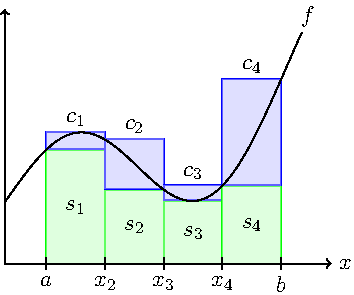
\includegraphics[scale=1.8]{asymptote/frpg}
			\end{figure}           
			\vspace{2 cm}
			\raggedleft Sindre Sogge Heggen   \end{center}
	\end{titlepage}
	\pagecolor{white}
\newpage
\phantom{}
\thispagestyle{empty}	
\newpage	
\import{kap0/}{framside}
\newpage

%\addcontentsline{toc}{chapter}{Innhold}
\footnotesize
\tableofcontents
\normalsize
\chapter{Følger og rekker\label{Folgerogrekker}}
\vspace{20pt}
\import{fol/}{fol}
\newpage
\import{opg/fol/}{opg}
\chapter{Trigonometri\label{Trigonometri}}
\vspace{20pt}
\import{tri/}{tri}
\newpage
\import{opg/tri/}{opg}
\newpage
\import{tri/}{cmt}
\chapter{Vektorer i rommet\label{Vektorerirommet}}
\vspace{20pt}
\import{vek/}{vekt}
\newpage
\import{opg/vek/}{opg}
\chapter{Romgeometrier\label{Romgeometrier}}
\vspace{20pt}
\import{rom/}{rom}
\newpage
\import{opg/rom/}{opg}
\chapter{Derivasjon\label{Derivasjon}}
\vspace{20pt}
\import{der/}{der}
\newpage
\import{opg/der/}{opg}
\chapter{Integrasjon \label{Integrasjon}}
\vspace{20pt}
\import{int/}{int}
\newpage
\subimport{opg/int/}{opg}
\chapter{Differensialligninger\label{Differensialligninger}}\
\vspace{20pt}
\import{dif/}{dif}
\newpage
\import{opg/dif/}{opg}
\titleformat{\chapter}[hang]
{\normalfont\LARGE\bfseries}{}{}{\vspace{-1cm}\Huge}
\chapter*{Vedlegg \ref{husksincos}-\ref{d} \label{Tips} \addcontentsline{toc}{chapter}{Vedlegg A-E}}
\phantomsection
\vspace{20 pt}
\import{tips/}{tips}
{\printindex \addtocontents{toc}{\protect\vspace{-5pt}}
	\addcontentsline{toc}{chapter}{Indeks}\phantomsection}
\chapter*{Fasit}
\setlength{\parskip}{5pt}
\addtocontents{toc}{\protect\vspace{-5pt}}
\addcontentsline{toc}{chapter}{Fasit}\phantomsection
\import{opg/fol/}{fas}
\import{opg/tri/}{fas}
\newpage
\import{opg/vek/}{fas}
\import{opg/rom/}{fas}
\import{opg/der/}{fas}
\import{opg/int/}{fas}
\import{opg/dif/}{fas}
\phantom{}
\newpage
\thispagestyle{empty}
\phantom{}
\newpage
\import{kap0/}{bakside}
%\thispagestyle{empty} 
%\phantom{}
\end{document}
%\end{document}











